\chapter{Analisi dei requisiti e progettazione}\label{ch:progettazione}
Le sezioni 2.1--2.6 e le appendici A--B sono proposte per revisione.
Le sezioni 2.7--2.8 restano esplicitamente provvisorie.
\begingroup
\emergencystretch=6em
\def\UrlBreaks{\do\a\do\b\do\c\do\d\do\e\do\f\do\g\do\h\do\i\do\j\do\k\do\l\do\m\do\n\do\o\do\p\do\q\do\r\do\s\do\t\do\u\do\v\do\w\do\x\do\y\do\z\do\A\do\B\do\C\do\D\do\E\do\F\do\G\do\H\do\I\do\J\do\K\do\L\do\M\do\N\do\O\do\P\do\Q\do\R\do\S\do\T\do\U\do\V\do\W\do\X\do\Y\do\Z}
\section{Diagramma dei casi d'uso}\label{sec:casi-uso}
La concessionaria offre tre percorsi: il cliente consulta l'offerta e avvia
operazioni; il venditore decide gli esiti delle richieste e la destinazione
dei veicoli; il manager mantiene catalogo, basi prezzo e sconti e legge il
registro economico. Le figure~\ref{fig:uc-cliente}--\ref{fig:uc-manager}
sono viste complementari dello stesso sistema. Le associazioni indicano
partecipazione, non ordine temporale o chiamate tra servizi.

Le ellissi azzurre rappresentano obiettivi applicativi (livello O).
\textbf{UC-04} \`e una sottofunzione applicativa (livello F) della vendita
al cliente UC-03: autorizza il successivo saldo, senza completare la vendita.
Le ellissi grigie raccolgono il supporto all'interazione (livello S):
registrazione, accesso, gestione dell'identit\`a e ricarica del conto demo.
L'accesso \`e una precondizione degli obiettivi autenticati, non un
\emph{include} da ripetere a ogni azione. La registrazione riguarda solo il cliente.

Il diverso livello è dichiarato nelle schede della sezione~\ref{sec:template} e dell'appendice~\ref{app:casi-uso}.
UC-03 e UC-05 attraversano sessioni e ruoli, mentre UC-01, UC-02 e UC-06
hanno un obiettivo pi\`u circoscritto. Le viste non simulano un'unica scala
di dettaglio: mantengono riconoscibili i casi principali e rendono esplicita
la loro scomposizione. In particolare, UC-05 compare sia per il cliente che
propone sia per il venditore che accetta o rifiuta.

La figura~\ref{fig:uc-autori} riprende \emph{Users SWE}, la tavola degli
autori, mantenendo attori, generalizzazioni, ellissi e disposizione d'insieme.
La registrazione \`e associata al solo cliente; la consultazione delle
prenotazioni del venditore, assente dall'interfaccia corrente, \`e rimossa.
Le funzioni comuni sono ereditate da \emph{Utente}; l'addebito incluso nei
due flussi \`e un comportamento interno, distinto dalla ricarica UC-S04.
Le due partecipazioni a UC-05 e le due parti di UC-09 non sono casi nuovi.
La tavola \`e su foglio A3 per conservarne la leggibilit\`a; le tre viste
seguenti ne dettagliano gli obiettivi per ruolo.
\tavolaautori{casi-uso-autori}{Casi d'uso: tavola degli autori corretta, con attori e struttura originali}{fig:uc-autori}

\begin{figure}[!htbp]\centering
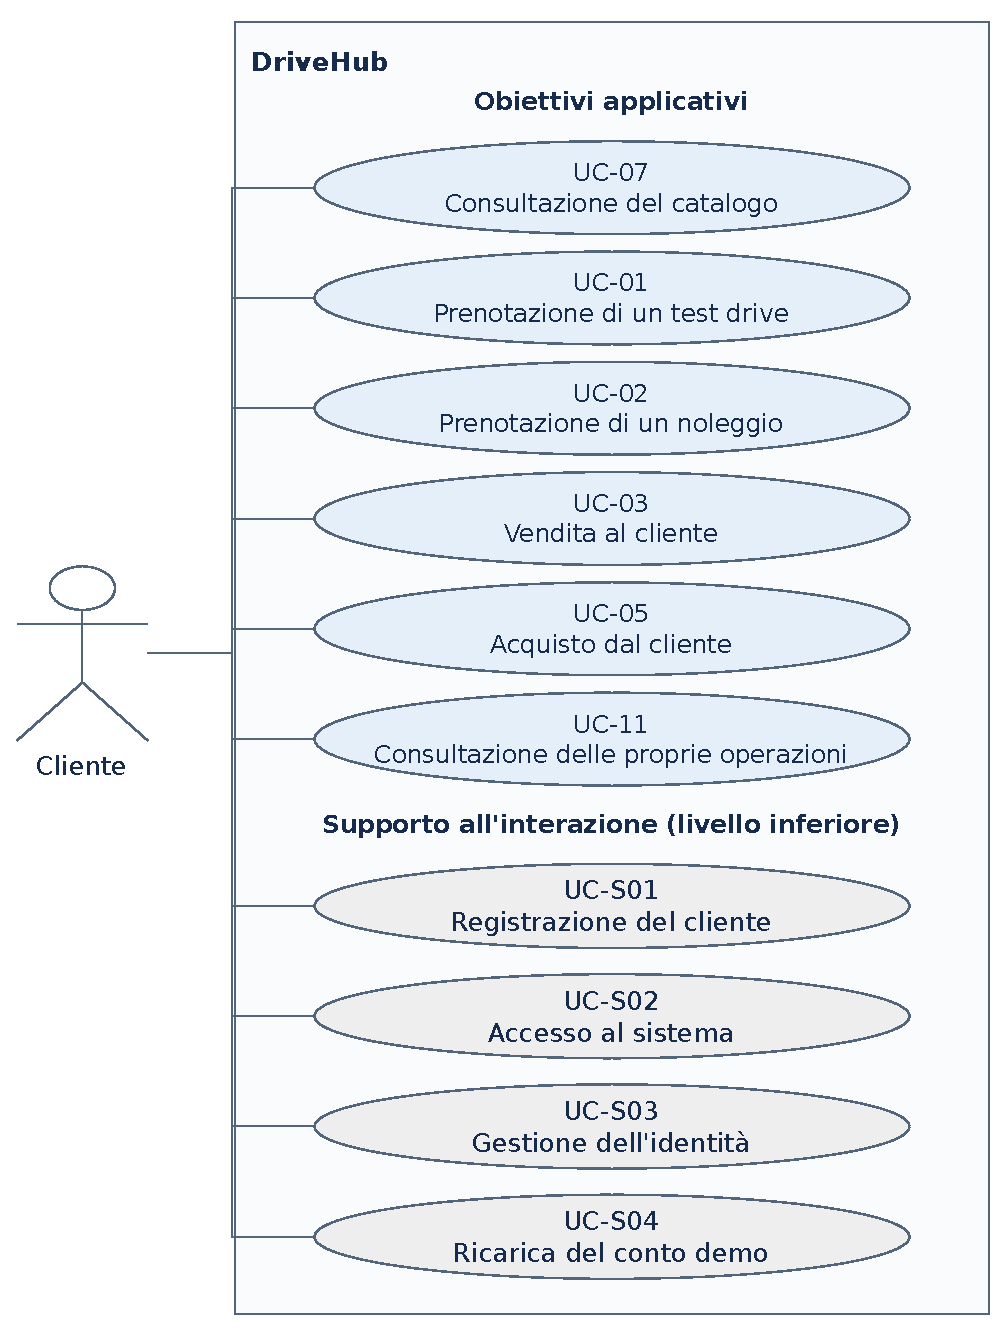
\includegraphics[width=\linewidth,height=.72\textheight,keepaspectratio]{diagrammi/casi-uso-cliente.drawio.pdf}
\caption{Cliente: obiettivi commerciali e consultazioni; in grigio le funzioni di supporto. UC-03 e UC-05 richiedono anche la partecipazione del venditore.}\label{fig:uc-cliente}
\end{figure}
\clearpage
\begin{figure}[!htbp]\centering
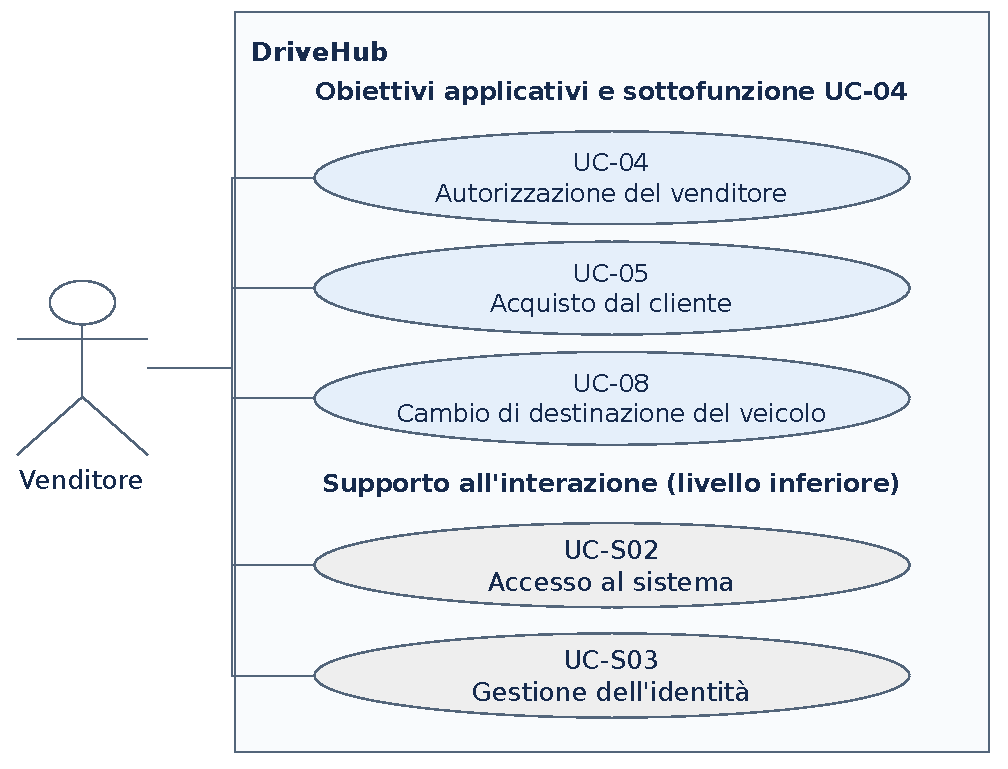
\includegraphics[width=.85\linewidth,height=.67\textheight,keepaspectratio]{diagrammi/casi-uso-venditore.drawio.pdf}
\caption{Venditore: autorizzazione della vendita al cliente (UC-04), esito dell'acquisto dal cliente (UC-05) e destinazione dell'inventario (UC-08).}\label{fig:uc-venditore}
\end{figure}
\begin{figure}[!htbp]\centering
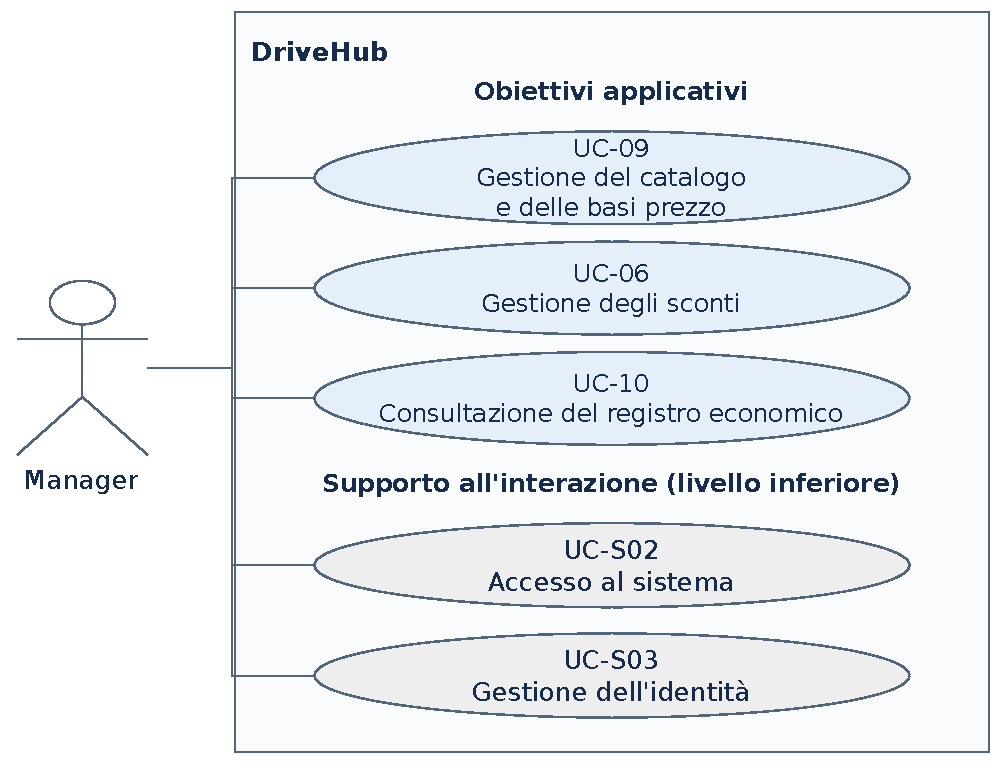
\includegraphics[width=.85\linewidth,height=.67\textheight,keepaspectratio]{diagrammi/casi-uso-manager.drawio.pdf}
\caption{Manager: manutenzione commerciale e consultazione del registro. Le identit\`a staff esistono gi\`a; non vi \`e una registrazione pubblica del personale.}\label{fig:uc-manager}
\end{figure}
\clearpage

\section{Template dei casi principali}\label{sec:template}
Le sei schede complete seguono il percorso originale: test drive, noleggio,
vendita al cliente, cessione, autorizzazione e sconti. UC-05 precede UC-04
nell'esposizione e conserva il proprio identificativo. Le nove schede
aggiuntive sono nell'appendice~\ref{app:casi-uso}.
\begingroup
\small
\setlist{itemsep=1pt,topsep=2pt}
% Schede riscontrate sul codice corrente; non costituiscono esiti di test.
\newcommand{\scheda}[7]{%
  \subsection{\texorpdfstring{\raggedright #1 --- #2}{#1 --- #2}}\label{uc:#1}
  \begin{longtable}{|p{.20\linewidth}|p{.72\linewidth}|}
  \caption{Scheda del caso d'uso #1}\\\hline
  \textbf{Campo} & \textbf{Contenuto}\\\hline\endfirsthead
  \textbf{Campo} & \textbf{Contenuto (continua)}\\\hline\endhead
  Identificativo & #1\\\hline
  Descrizione & #3\\\hline
  Livello & #4\\\hline
  Attori & #5\\\hline
  Precondizioni & #6\\\hline
  Postcondizioni & #7\\\hline
  \end{longtable}
}
\newcommand{\principale}{\paragraph{Flusso principale}}
\newcommand{\alternative}{\paragraph{Alternative}}

Ogni titolo riporta identificativo stabile e denominazione. Le alternative
\emph{n.a}, \emph{n.b} si diramano dal passo \emph{n} della stessa scheda;
si indica se il caso riprende o termina. O indica un obiettivo applicativo,
F una sottofunzione applicativa e S una funzione di supporto. Sono livelli
descrittivi, non livelli di autorizzazione. Gli attori sono ruoli dell'interfaccia;
non si assume un controllo dei permessi indipendente in ogni servizio.
Le postcondizioni descrivono il successo; in caso di errore transazionale
le scritture della singola operazione vengono annullate. Un errore successivo
nell'aggiornamento della vista non annulla un'operazione gi\`a confermata.


Le prove richiamate sono sorgenti e risultati storici, non nuove esecuzioni.
\clearpage
\scheda{UC-01}{Prenotare un test drive}
{Il cliente riserva un giro di prova di un'ora su un veicolo della concessionaria.}
{O --- obiettivo applicativo.}
{Cliente; indirettamente altri clienti con prenotazioni concorrenti.}
{Cliente autenticato; veicolo visibile nel catalogo vendita o noleggio.}
{Prenotazione associata a cliente, veicolo e data/ora; nessun addebito.}
\principale
\begin{enumerate}
\item Il cliente seleziona un veicolo in \emph{Auto in Vendita} o \emph{Auto a Noleggio}.
\item Apre \emph{Prenota Test Drive}, sceglie data e ora iniziale e conferma.
      La UI propone ore intere dalle 09:00 alle 16:00.
\item Il servizio rilegge il veicolo, ammette solo \code{SALE}/\code{RENT},
      controlla che l'istante non sia passato, che il cliente abbia meno di tre
      test drive attivi e che slot e giorno non siano occupati da test drive o noleggi incompatibili.
\item Il sistema salva la prenotazione nella transazione e aggiorna \emph{Le Mie Operazioni}.
\item Il cliente legge la conferma con data e ora del giro di prova.
\end{enumerate}
\alternative
\begin{description}
\item[2.a] Annullamento del dialogo: nessuna prenotazione; termina.
\item[3.a] Data passata, stato cambiato, limite raggiunto o indisponibilit\`a:
  errore, nessuna nuova prenotazione; il cliente pu\`o ripartire da 1 o 2.
\item[4.a] Errore di persistenza: rollback della prenotazione; termina senza successo.
\item[5.a] Successivamente il cliente seleziona un proprio test drive in
  \emph{Le Mie Operazioni} e lo annulla: viene rimosso e la tabella aggiornata.
  Un identificativo non appartenente al cliente viene rifiutato.
\item[5.b] Un successivo noleggio o completamento di vendita sul veicolo
  cancella tutti i suoi test drive futuri, anche fuori dal periodo noleggiato.
  Lo storico rimane; la cancellazione partecipa alla transazione commerciale.
\end{description}
\begin{flushleft}\textbf{Riscontro:} \code{TestDriveService}, \code{TestDriveCancellationObserver},
\code{ClientDashboardView}. La durata \`e una convenzione del giro di prova;
la UI seleziona ore intere, senza attribuire al servizio un vincolo generale
sui minuti che il codice non applica per tutte le ore.\end{flushleft}


\begin{flushleft}\noindent\textbf{Prove e portata:} \code{BookingRulesTest} (fascia e date), \code{BookingConcurrencyIntegrationTest} (limite, slot concorrenti e rollback), \code{TestDriveCancellationIntegrationTest} (cancellazioni); evidenze storiche \code{r06-bookings}/\code{r11-integrated}.\end{flushleft}
\clearpage
\scheda{UC-02}{Noleggiare un veicolo}
{La concessionaria prenota un proprio veicolo al cliente e incassa subito il costo del periodo.}
{O --- obiettivo applicativo.}
{Cliente; clienti titolari di test drive futuri sul medesimo veicolo.}
{Cliente autenticato con conto demo; veicolo presente nel catalogo noleggio.}
{Noleggio salvato e costo intero addebitato; test drive futuri del veicolo cancellati;
il veicolo conserva la destinazione \code{RENT}.}
\principale
\begin{enumerate}
\item Il cliente seleziona un veicolo in \emph{Auto a Noleggio} e apre \emph{Prenota Noleggio}.
\item Sceglie inizio e fine; il dialogo mostra il costo del periodo con estremi inclusi.
\item Conferma. Il servizio rilegge stato, disponibilit\`a e prezzo: inizio non passato,
      fine non precedente all'inizio, stato \code{RENT}, nessuna sovrapposizione.
\item Il sistema verifica il conto e addebita il 100\% del costo ricalcolato.
\item Salva il noleggio e cancella tutti i test drive futuri del veicolo,
      anche oltre il periodo prenotato, nella stessa transazione.
\item Mostra la conferma e aggiorna saldo e operazioni del cliente.
\end{enumerate}
\alternative
\begin{description}
\item[2.a] Date incomplete o invertite: il preventivo non \`e valido;
  il cliente corregge il periodo al passo 2 oppure annulla senza effetti.
\item[3.a] Stato cambiato o periodo gi\`a occupato, anche per una prenotazione concorrente:
  rifiuto senza addebito; ripartire da 1 o 2.
\item[4.a] Conto assente o saldo insufficiente: nessun noleggio e nessun addebito; termina.
\item[5.a] Errore nel salvataggio o nelle cancellazioni collegate: rollback
  anche dell'addebito; nessun successo parziale.
\item[6.a] In seguito UC-08 destina il veicolo alla vendita: se non vi sono
  noleggi in corso, quelli con inizio futuro sono rimossi e rimborsati al 100\%.
  Il cliente vede l'effetto ricaricando le proprie operazioni.
\end{description}
\begin{flushleft}\textbf{Riscontro:} \code{RentalService}, \code{PriceCalculatorService},
\code{TestDriveCancellationObserver}. Il preventivo non \`e un accordo fissato:
il costo viene ricalcolato alla prenotazione. La UI non offre una cancellazione
autonoma del noleggio al cliente.\end{flushleft}


\begin{flushleft}\noindent\textbf{Prove e portata:} \code{BookingConcurrencyIntegrationTest} (conflitti e addebito), \code{TestDriveCancellationIntegrationTest} (rollback Observer), \code{VehicleDestinationIntegrationTest} (rimborsi); evidenze \code{r06-bookings}/\code{r06-destination}/\code{r11-integrated}.\end{flushleft}
\clearpage
\scheda{UC-03}{Richiedere e completare una vendita al cliente}
{La concessionaria vende un veicolo: acconto, autorizzazione del venditore e saldo del totale concordato.}
{O --- obiettivo applicativo articolato in pi\`u sessioni.}
{Cliente principale; venditore per UC-04.}
{Cliente autenticato con conto demo; veicolo proposto in vendita.}
{Nel successo completo: totale registrato come vendita al cliente,
richiesta rimossa, veicolo \code{SOLD}; test drive futuri cancellati.
Dopo il solo acconto: richiesta \code{SALE} aperta, totale fissato e veicolo \code{BLOCKED}.}
\principale
\begin{enumerate}
\item Il cliente seleziona il veicolo in \emph{Auto in Vendita} e avvia l'acquisto.
\item Legge prezzo indicativo e acconto del 20\% nel dialogo e conferma.
\item Il servizio riserva il veicolo solo se ancora \code{SALE}, ricalcola il prezzo,
  addebita l'acconto e salva la richiesta con totale concordato, senza venditore n\'e scadenza.
\item Il venditore approva la richiesta attraverso UC-04, fissando il termine di un mese.
\item Il cliente seleziona la richiesta approvata in \emph{Le Mie Operazioni},
  apre il pagamento del saldo e conferma il residuo del totale concordato.
\item Il servizio verifica autorizzazione e scadenza, addebita il residuo,
  registra l'intero totale nel registro, elimina la richiesta e porta il veicolo a \code{SOLD}.
  Cancella i test drive futuri nella stessa transazione del saldo.
\end{enumerate}
\alternative
\begin{description}
\item[2.a] Annullamento: il veicolo non viene riservato; termina.
\item[3.a] Veicolo non pi\`u disponibile, conto assente o fondi insufficienti:
  rollback di acconto, richiesta e stato; termina.
\item[4.a] Rifiuto del venditore: rimborso integrale dell'acconto,
  richiesta eliminata e veicolo di nuovo \code{SALE}; termina.
\item[5.a] Richiesta non autorizzata o gi\`a scaduta: il saldo viene rifiutato.
  Annullare il dialogo lascia invece aperta la richiesta.
\item[6.a] Saldo insufficiente o errore transazionale: nessuna vendita completata;
  restano acconto e richiesta precedenti; il cliente pu\`o riprovare entro il termine.
\item[6.b] Mancato saldo entro il termine: all'accesso successivo il controllo
  delle scadenze trattiene il 20\% dell'acconto come penale, restituisce il resto,
  rimuove la richiesta e libera il veicolo per la vendita. Non \`e un processo periodico in background.
\end{description}
\begin{flushleft}\textbf{Riscontro:} \code{PurchaseService}, \code{Request}, ADR 0001.
Acconto e saldo hanno transazioni distinte. Basi e sconti successivi non
modificano il totale gi\`a concordato; la penale \`e il 20\% dell'acconto, non del totale.\end{flushleft}


\begin{flushleft}\noindent\textbf{Prove e portata:} \code{PurchaseAgreementIntegrationTest} (accordo immutato, autorizzazione, scadenza, fondi e rollback), \code{TestDriveCancellationIntegrationTest} (Observer); evidenze \code{r04-agreement}/\code{r11-integrated}.\end{flushleft}
\clearpage
\scheda{UC-05}{Proporre un veicolo alla concessionaria}
{La concessionaria valuta e acquista il veicolo ceduto dal cliente; l'etichetta UI \emph{Vendi la tua Auto} usa il punto di vista del cliente.}
{O --- obiettivo applicativo in due fasi, proposta ed esito.}
{Cliente proponente; venditore che decide.}
{Cliente autenticato; modello gi\`a censito; dati del veicolo disponibili.
Se il VIN \`e noto, stato \code{SOLD}, ultima vendita al proponente e nessuna richiesta aperta.}
{Accettazione: stima accreditata al cliente, acquisto della concessionaria registrato,
richiesta rimossa e veicolo \code{SALE}. Dopo la proposta: veicolo \code{WAITING} e richiesta \code{PURCHASE}.}
\principale
\begin{enumerate}
\item Il cliente apre \emph{Vendi la tua Auto} e indica marchio, modello,
  VIN, targa, chilometri e anno.
\item Pu\`o calcolare il preventivo, basato sul modello e sui dati inseriti.
\item Invia la proposta. Il servizio valida i dati e l'eventuale titolarit\`a
  del VIN noto; crea il veicolo oppure aggiorna quello gi\`a venduto al cliente.
\item Salva il veicolo \code{WAITING} e la richiesta con stima ricalcolata,
  positiva o nulla, senza effettuare pagamenti.
\item Il venditore seleziona la proposta \emph{Acquisto dal cliente} in
  \emph{Richieste in Sospeso} e aziona \emph{Approva Richiesta}.
\item Il sistema accredita la stima memorizzata, registra l'acquisto dal cliente
  con venditore, porta il veicolo a \code{SALE} ed elimina la richiesta,
  nella stessa transazione. La UI mostra l'esito.
\end{enumerate}
\alternative
\begin{description}
\item[2.a] Preventivo non richiesto: il cliente pu\`o passare direttamente a 3;
  il servizio ricalcola comunque la stima all'invio.
\item[3.a] Dati invalidi, anno precedente al modello, VIN occupato o non
  appartenente al proponente, richiesta gi\`a aperta: errore e nessuna nuova proposta;
  correggere al passo 1.
\item[5.a] Rifiuto: nessun accredito; richiesta eliminata.
  Il veicolo senza operazioni associate viene eliminato; con storico torna \code{SOLD}.
\item[6.a] Stima nulla, conto mancante, richiesta non pi\`u valida o errore di persistenza:
  rollback dell'intero esito, senza pagamento o acquisizione parziali.
\end{description}
\begin{flushleft}\textbf{Riscontro:} \code{SaleToDealershipService},
\code{ClientDashboardView}, \code{SalesmanDashboardView}. Il registro conserva
un importo non negativo con tipo acquisto; il suo significato \`e un esborso
per la concessionaria. Non esiste un successivo pagamento a saldo per la cessione.
La proposta ammette una stima nulla, ma il conto rifiuta l'accredito zero:
l'accettazione fallisce con rollback (sezione~\ref{sec:sequenze}).\end{flushleft}


\begin{flushleft}\noindent\textbf{Prove e portata:} \code{SaleProposalIntegrationTest} (titolarità e VIN), \code{SaleOutcomeIntegrationTest} (accredito, storico, concorrenza e rollback); evidenze \code{r05-sale-outcome}/\code{r11-integrated}.\end{flushleft}
\clearpage
\scheda{UC-04}{Autorizzare una richiesta di vendita al cliente}
{Il venditore decide l'esito della richiesta con cui la concessionaria vender\`a un veicolo al cliente.}
{F --- sottofunzione applicativa di UC-03, svolta dal venditore.}
{Venditore principale; cliente destinatario dell'esito.}
{Venditore autenticato; richiesta \code{SALE} in sospeso, con acconto gi\`a versato e veicolo riservato.}
{Approvazione: richiesta attribuita al venditore e scadenza impostata a un mese da oggi;
il saldo resta da pagare e il veicolo rimane \code{BLOCKED}.}
\principale
\begin{enumerate}
\item Il venditore apre \emph{Richieste in Sospeso}.
\item Seleziona una riga \emph{Vendita al cliente}, verificando totale,
  acconto e residuo mostrati nella tabella.
\item Aziona \emph{Approva Richiesta}; non compare una conferma preventiva.
\item Il servizio rilegge la richiesta, verifica che sia \code{SALE},
  assegna il venditore e la scadenza a un mese dalla data corrente.
\item La UI mostra l'esito e ricarica richieste e inventario;
  il cliente potr\`a saldare in UC-03.
\end{enumerate}
\alternative
\begin{description}
\item[2.a] Nessuna riga selezionata: messaggio di selezione mancante; ritorno a 2.
\item[2.b] Riga \emph{Acquisto dal cliente}: non \`e questa autorizzazione;
  la stessa azione conclude la cessione secondo UC-05.
\item[3.a] \emph{Rifiuta Richiesta}: il servizio restituisce l'intero acconto,
  elimina la richiesta e ripristina \code{SALE} nella stessa transazione.
  La vendita non prosegue; nessuna penale.
\item[4.a] Richiesta rimossa o tipo non valido: errore, nessuna nuova autorizzazione;
  il venditore ricarica l'elenco.
\item[4.b] Errore durante l'aggiornamento oppure durante il rimborso di 3.a:
  rollback della decisione; lo stato precedente rimane valido.
\end{description}
\begin{flushleft}\textbf{Riscontro:} \code{SalesmanDashboardView},
\code{PurchaseService.approvePurchase}, \code{PurchaseService.rejectPurchase},
\code{OperationQueryService}. Il caso non registra un nuovo venditore e non
rappresenta l'abilitazione di un account staff. La selezione delle richieste
in sospeso \`e affidata alla query della UI; non si attribuisce al comando
un controllo aggiuntivo contro ogni possibile riapprovazione da un chiamante diverso.\end{flushleft}


\begin{flushleft}\noindent\textbf{Prove e portata:} \code{PurchaseAgreementIntegrationTest} (approvazione e termine), \code{PurchaseConcurrencyIntegrationTest} (rifiuto, rimborso ed esiti concorrenti); l\'assenza di selezione e la riapprovazione non sono certificate da quel test. Evidenze \code{r04-agreement}/\code{r11-integrated}.\end{flushleft}
\clearpage
\scheda{UC-06}{Gestire lo sconto su un veicolo}
{Il manager applica o rimuove una promozione di modello o di singolo veicolo.}
{O --- obiettivo applicativo di gestione commerciale.}
{Manager; clienti interessati ai nuovi prezzi.}
{Manager autenticato; modello o veicolo destinatario gi\`a presente nel catalogo.}
{Sconto salvato o rimosso e tabella aggiornata. I nuovi calcoli usano il massimo
fra sconto modello e veicolo; i totali concordati nelle richieste aperte restano invariati.}
\principale
\begin{enumerate}
\item Il manager apre la scheda \emph{Sconti}.
\item Nel riquadro modello seleziona un modello; nel riquadro veicolo
  inserisce invece l'identificativo del veicolo.
\item Inserisce una percentuale intera tra 0 e 50 e aziona \emph{Salva} nel riquadro scelto.
\item Il servizio valida la percentuale e persiste lo sconto;
  uno sconto gi\`a presente sullo stesso elemento viene aggiornato.
\item La UI mostra la conferma e ricarica le due tabelle degli sconti.
\end{enumerate}
\alternative
\begin{description}
\item[2.a] Modello non selezionato o ID non numerico: errore prima del salvataggio;
  ritorno a 2. Un ID veicolo inesistente viene rifiutato dalla persistenza.
\item[3.a] Percentuale non intera o esterna a 0--50: errore, nessuna modifica; ritorno a 3.
\item[3.b] Il manager seleziona uno sconto esistente e aziona \emph{Rimuovi}:
  il servizio elimina lo sconto e la tabella viene ricaricata.
  Senza selezione l'azione non modifica dati; non compare una conferma preventiva.
\item[4.a] Errore transazionale: nessun nuovo sconto salvato; termina senza successo.
\item[5.a] Un'altra tabella gi\`a aperta mostra ancora il vecchio prezzo:
  ricaricarla con \emph{Aggiorna} oppure riaprire la vista.
  La UI non propaga automaticamente ogni modifica a tutte le dashboard gi\`a aperte.
\end{description}
\begin{flushleft}\textbf{Riscontro:} \code{CatalogService}, \code{Discount},
\code{PriceCalculatorService}, \code{ManagerDashboardView}. Gli sconti non
si sommano. La base manuale del veicolo sostituisce la base del modello nella
stessa formula; non impone un prezzo finale sottratto agli sconti.\end{flushleft}


\begin{flushleft}\noindent\textbf{Prove e portata:} \code{PriceCalculatorServiceTest} (massimo e base manuale), \code{DomainInvariantsTest} (0--50), \code{PriceSelectionIntegrationTest} (persistenza della base); evidenze \code{r03-prices}/\code{r11-integrated}.\end{flushleft}

\endgroup
\clearpage
\noindent\textbf{Tracciabilit\`a verso interfaccia e servizi.}
I nomi UI possono usare il punto di vista del cliente: \emph{Acquista Veicolo}
avvia una vendita della concessionaria, mentre \emph{Vendi la tua Auto}
avvia un acquisto dal cliente. Nelle richieste, \code{SALE} e \code{PURCHASE}
mantengono questi significati. Il registro distingue inoltre \code{PENALTY};
un importo positivo non basta da solo a stabilire la direzione economica.

\begin{description}[style=nextline]\raggedright
\item[UC-01, UC-02 e UC-03.]
\code{ClientDashboardView} apre cataloghi, dialoghi e operazioni;
\code{TestDriveService}, \code{RentalService} e \code{PurchaseService}
eseguono i rispettivi comandi. La dashboard avvia il controllo delle
scadenze all'accesso del cliente, senza un pianificatore periodico.
\item[UC-04 e UC-05.]
\code{SalesmanDashboardView} distingue i due tipi di richiesta.
\code{PurchaseService} governa l'autorizzazione e il saldo della vendita;
\code{SaleToDealershipService} governa proposta ed esito della cessione.
\item[UC-06.]
\code{ManagerDashboardView} usa \code{CatalogService} per gli sconti;
\code{PriceCalculatorService} applica la formula. La base manuale
sostituisce la base del modello nella stessa formula (ADR 0001).
\end{description}

Completano le viste UC-07 (catalogo, scheda~\ref{uc:UC-07}), UC-08
(destinazione, scheda~\ref{uc:UC-08}), UC-09 (manutenzione catalogo e basi,
scheda~\ref{uc:UC-09}), UC-10 (registro, scheda~\ref{uc:UC-10}) e UC-11
(proprie operazioni, scheda~\ref{uc:UC-11}). Il supporto comprende UC-S01
(registrazione, scheda~\ref{uc:UC-S01}), UC-S02 (accesso,
scheda~\ref{uc:UC-S02}), UC-S03 (identit\`a, scheda~\ref{uc:UC-S03}) e
UC-S04 (ricarica demo, scheda~\ref{uc:UC-S04}). Ogni identificativo conserva
lo stesso significato nei diagrammi, nelle schede e nella navigazione.

La separazione delle transazioni spiega gli stati intermedi: dopo l'acconto
la vendita non \`e ancora conclusa; dopo una proposta di cessione il cliente
non \`e ancora pagato. Gli esiti osservati nelle schermate illustrano il
percorso, mentre le regole qui dichiarate derivano anche dal riscontro dei
sorgenti. Non si attribuisce a questo ticket una nuova certificazione della
concorrenza o dei rollback tramite test applicativi.
\clearpage

\section{Mockups}\label{sec:mockups}
Il titolo concordato \`e mantenuto; le figure sono \textbf{screenshot
dell'applicazione JavaFX realmente eseguita il 12 novembre 2026}, non
ricostruzioni grafiche. L'avvio usa \code{App.start}, le viste e il tema
correnti, con rendering software su Xvfb e PostgreSQL 16 dedicato.
I nomi e gli importi provengono dalla fixture dimostrativa. Solo nel database
temporaneo sono state spostate alcune date per mostrare operazioni ancora
valide; schema, demo SQL e archivi operativi non sono stati modificati.
Le immagini originali, a risoluzione piena, sono conservate in
\code{docs/relazione/screenshot}; non sono prove di tutte le alternative.

\newcommand{\schermata}[3]{%
  \begin{figure}[!htbp]\centering
  \includegraphics[width=\linewidth,height=.37\textheight,keepaspectratio]{screenshot/#1.png}
  \caption{#2}\label{fig:#3}
  \end{figure}}

\subsection{Autenticazione}
Accesso comune ai tre ruoli (UC-S02) e registrazione riservata al cliente
(UC-S01); il ruolo deriva dall'identità autenticata.

\subsubsection{Schermata iniziale}
\code{App.start} apre direttamente \code{LoginView}. Non esiste una
Welcome Page separata: \emph{Accedi} e \emph{Registrati} sono le due tab
della stessa vista. All'ingresso non si mostrano cataloghi né si seleziona
un ruolo. La figura~\ref{fig:ui-accesso} documenta anche questo punto del
percorso originale, senza duplicare un'immagine o inventare una pagina.

\subsubsection{Accesso}
Il form raccoglie email e password; \emph{Accedi} invoca \code{AuthService}.
Credenziali accettate aprono la dashboard del sottotipo utente, mentre
un errore lascia la vista di accesso e mostra il messaggio. Non vi è una
scelta pubblica del ruolo. Il logout da ogni dashboard ritorna qui.
\schermata{01-accesso}{Accesso corrente, coincidente con la schermata iniziale: email e password.}{ui-accesso}

\subsubsection{Registrazione}
Il cliente inserisce nome, cognome, email e password.
\emph{Crea Account Cliente} valida i dati, crea identità e conto demo a saldo zero nella
stessa transazione e apre la dashboard cliente. Email già utilizzata o dati
invalidi producono un errore; il form rimane disponibile per la correzione.
Venditori e manager sono predisposti nel DB: il precedente selettore di ruolo
non ha un equivalente corrente.
\schermata{02-registrazione}{Registrazione del solo cliente e creazione congiunta del conto demo.}{ui-registrazione}
\clearpage

\subsection{Area Customer}
Le etichette \emph{Customer} e \emph{Salesman} restano nei titoli concordati;
nel testo si usano cliente e venditore. Le quattro tab sono \emph{Auto in
Vendita}, \emph{Auto a Noleggio}, \emph{Vendi la tua Auto} e \emph{Le Mie Operazioni}.

\subsubsection{Catalogo veicoli}
I due cataloghi mostrano modello, anno, targa/usato, chilometri, base
applicata, prezzo consigliato ed effettivo; per il noleggio si mostra anche
la tariffa iniziale giornaliera. Il cliente seleziona una riga e avvia
acconto, noleggio o test drive con i comandi della tab. \emph{Aggiorna}
rilegge disponibilità e prezzi; il comando commerciale li ricontrolla alla
conferma. Durante le letture asincrone i dati sono disabilitati; un errore
espone \emph{Riprova}. La selezione mancante non avvia l'operazione.
Non si attribuiscono alla vista i vecchi filtri testuali non presenti.
\schermata{03-cliente-catalogo}{Catalogo vendita: selezione, acconto del 20\% e test drive.}{ui-cliente-catalogo}
\schermata{05-cliente-noleggio}{Catalogo noleggio: tariffa iniziale e azioni sul veicolo selezionato.}{ui-cliente-noleggio}
\clearpage

\subsubsection{Vendite al cliente e richieste}
\emph{Le Mie Operazioni} mostra le richieste del cliente con veicolo,
totale concordato, acconto, residuo, autorizzazione e scadenza. Selezionare
la richiesta e confermare il saldo completa UC-03 solo dopo UC-04 e nel
termine. Il servizio usa l'accordo persistito, anche dopo variazioni di
listino; fondi insufficienti lasciano valida la richiesta. Chiudere il
dialogo non annulla l'acconto. Non esiste il vecchio comando del cliente
per annullare autonomamente l'acquisto con penale: rifiuto e scadenza hanno
i percorsi distinti descritti nella scheda. La vista non è un registro
completo delle compravendite concluse; quel registro è del manager.
\schermata{08-cliente-operazioni}{Le Mie Operazioni: richieste, noleggi e test drive del cliente; saldo e annullamento del test drive.}{ui-cliente-operazioni}

\subsubsection{Noleggi e test drive}
Le prenotazioni partono dal catalogo e aprono dialoghi, non una vecchia
scheda unica di inserimento. Il test drive richiede data e ora; la UI
propone ore intere 09:00--16:00. \emph{Conferma} salva senza addebito,
se stato, fascia, limite di tre attivi e conflitti lo consentono.
Il noleggio richiede inizio e fine, mostra un preventivo e addebita il
100\% del costo ricalcolato alla conferma, con estremi inclusi.
Annullare un dialogo non scrive dati. Prenotazioni e annullamento del solo
test drive si trovano in \emph{Le Mie Operazioni}
(figura~\ref{fig:ui-cliente-operazioni}); il cliente non può annullare da
qui un noleggio. Un impegno commerciale cancella tutti i test drive futuri
del veicolo, anche esterni al periodo noleggiato.
\schermata{04-cliente-dialogo-test-drive}{Dialogo del test drive: data, ora iniziale, conferma o annullamento.}{ui-test-drive}
\schermata{06-cliente-dialogo-noleggio}{Dialogo di noleggio: periodo e preventivo, ricalcolato al comando finale.}{ui-noleggio}
\clearpage

\subsubsection{Proposta di cessione del proprio veicolo}
In \emph{Vendi la tua Auto} il cliente sceglie marchio e modello censiti e
inserisce VIN, targa, chilometri e anno. \emph{Calcola Preventivo} mostra la
stima; è facoltativo. \emph{Invia Proposta di Vendita} ricalcola e persiste
la stima con veicolo \code{WAITING} e richiesta \code{PURCHASE}, senza
accredito. Dati invalidi o VIN noto senza titolarità sono rifiutati.
L'esito del venditore conclude UC-05: per la concessionaria è un acquisto
dal cliente. Una stima nulla può essere proposta ma non accreditata.
\schermata{07-cliente-cessione}{Proposta di cessione: dati del veicolo, preventivo e invio al venditore.}{ui-cessione}

\subsubsection{Conto dimostrativo}
Il saldo compare nell'header; il dialogo comune mostra anche IBAN e saldo attuale. \emph{Ricarica Saldo} apre la richiesta di un
importo positivo e aggiorna il saldo dopo la scrittura; un valore invalido
non produce una ricarica. La stessa funzione è una tab del dialogo
\emph{Gestione Account} (figura~\ref{fig:ui-identita}). Non è una scheda
bancaria dedicata: la UI corrente non offre il prelievo autonomo né una
connessione bancaria reale. Il conto serve agli addebiti e accrediti
delle operazioni dimostrative e non conserva un estratto di ogni movimento.

\subsubsection{Profilo}
\emph{Gestione Account} apre \code{AccountManagementDialog}, comune ai
ruoli. Nuova email o nuova password richiedono la password corrente;
il successo aggiorna l'identità e chiude il dialogo, un errore lo lascia
aperto. L'eliminazione richiede password e conferma definitiva; se riesce
ritorna all'accesso. Riferimenti storici possono impedirla; un conto
positivo non è di per sé una protezione dalla cancellazione del cliente.
\schermata{09-cliente-identita}{Dialogo comune di gestione identità: qui aperto dal cliente, con la tab aggiuntiva di ricarica.}{ui-identita}
\clearpage

\subsection{Area Salesman}
Le sole tab sono \emph{Richieste in Sospeso} e \emph{Gestione Stato Inventario}.
La tipologia della riga distingue UC-04 dall'esito di UC-05.

\subsubsection{Proposte di cessione in attesa}
Il venditore seleziona una richiesta \emph{Acquisto dal cliente}
(\code{PURCHASE}) nella tabella comune, riconoscendola dalla tipologia;
non c'è una tab separata né si deve presumere un filtro dedicato.
\emph{Approva Richiesta} accredita la stima persistita, registra l'acquisto
con il venditore e rende il veicolo \code{SALE}. \emph{Rifiuta Richiesta}
non paga: elimina il veicolo nuovo o ripristina \code{SOLD} se ha storico.
Nessuna selezione produce un messaggio; errori nel comando causano rollback.
\schermata{10-venditore-richieste}{Tabella comune delle richieste SALE e PURCHASE, con importi e comandi di esito.}{ui-venditore-richieste}

\subsubsection{Richieste di vendita al cliente}
Nella stessa figura~\ref{fig:ui-venditore-richieste}, la riga \code{SALE}
espone totale, acconto e residuo. \emph{Approva Richiesta} assegna venditore
e termine di un mese; non incassa il saldo. \emph{Rifiuta Richiesta}
rimborsa tutto l'acconto e libera il veicolo, senza penale. Non compare una
conferma preventiva di approvazione/rifiuto. Il cliente completa poi UC-03
nella propria area. La lista mostra le richieste in sospeso; il comando di
approvazione non è una garanzia generale contro la riapprovazione diretta.

\subsubsection{Stato dei veicoli}
Il venditore seleziona nell'inventario un veicolo \code{SALE}/\code{RENT}
e conferma il cambio destinazione. La UI avvisa dei noleggi futuri;
il servizio rilegge sotto lock lo stato effettivo. Un noleggio in corso
impedisce il passaggio a vendita; i futuri sono eliminati e rimborsati
integralmente nella medesima transazione. Non è un editor di ogni stato
del veicolo: riserve, proposte e vendite hanno i propri comandi.
\schermata{11-venditore-inventario}{Inventario e cambio della sola destinazione vendita/noleggio.}{ui-venditore-inventario}

\subsubsection{Panoramica prenotazioni: limite attuale}
La vecchia panoramica di noleggi e test drive del venditore non ha un
equivalente corrente. Le sue due tab non offrono questa consultazione;
le prenotazioni personali sono del cliente. Si conserva il punto del
percorso originale dichiarando il limite, senza una figura storica
presentata come attuale o una nuova funzionalità implicita.

\subsubsection{Profilo}
Il pulsante \emph{Gestione Account} della dashboard apre lo stesso
\code{AccountManagementDialog}: modifica email/password con password
corrente ed eliminazione confermata, senza tab di ricarica. L'apertura
è riscontrata in \code{SalesmanDashboardView.buildUi}; non è stata
acquisita una nuova schermata staff. La figura~\ref{fig:ui-identita}
illustra il dialogo comune nel contesto cliente e non certifica una tab
Profilo separata del venditore. La coppia ID/ruolo indirizza le scritture;
le FK dello storico possono impedire l'eliminazione.
\clearpage

\subsection{Area Manager}
Le cinque tab sono \emph{Marchi}, \emph{Modelli}, \emph{Veicoli},
\emph{Sconti} e \emph{Registro economico}. I form modificano la stessa
vista, senza una pagina di dettaglio separata. L'esposizione segue
parco veicoli, marche/modelli, registro e profilo come nell'originale.

\subsubsection{Parco veicoli}
La tab \emph{Veicoli} mostra catalogo e prezzi. Il form raccoglie modello,
VIN, targa, chilometri, anno, destinazione iniziale \code{SALE}/\code{RENT} e scelta della base; una base manuale sostituisce
quella del modello nella stessa formula (ADR 0001), non il prezzo finale.
La selezione di un veicolo permette inoltre di scegliere modalità e base e usare \emph{Applica base alla selezione}. Inserimento e rimozione aggiornano l'elenco; dati invalidi o riferimenti
incompatibili producono errori. Gli sconti individuali sono oggi nella tab
\emph{Sconti}: ID veicolo e percentuale intera 0--50, con \emph{Salva} e
\emph{Rimuovi}. La rimozione è diretta, senza conferma preventiva.
Il massimo tra sconto veicolo e modello vale per nuovi calcoli; non cambia
un totale già concordato. Una tab già caricata può richiedere \emph{Aggiorna}.
\schermata{14-manager-veicoli}{Parco veicoli: basi applicate e scelta automatica/manuale.}{ui-manager-veicoli}
\schermata{15-manager-sconti}{Tab Sconti: gestione distinta dello sconto sul modello e sul veicolo.}{ui-manager-sconti}
\clearpage

\subsubsection{Marche e modelli}
Le anagrafiche occupano due tab. \emph{Marchi} riceve il nome e offre
aggiunta e rimozione della riga selezionata. \emph{Modelli} richiede marchio,
nome unico, base del modello e anno di rilascio. I comandi aggiornano le
tabelle; selezioni mancanti, anni invalidi e dipendenze esistenti impediscono
le operazioni incompatibili. Lo sconto di modello è gestito nell'altro
riquadro della tab \emph{Sconti} (figura~\ref{fig:ui-manager-sconti}): si
seleziona il modello e si salva o rimuove la percentuale 0--50. Non coincide
con lo sconto sul singolo esemplare e non si somma a esso.
\schermata{12-manager-marchi}{Anagrafica dei marchi: inserimento e rimozione.}{ui-manager-marchi}
\schermata{13-manager-modelli}{Anagrafica dei modelli: marchio, base e anno di rilascio.}{ui-manager-modelli}
\clearpage

\subsubsection{Registro delle operazioni}
La tab di sola consultazione legge le righe del registro: vendita al
cliente \code{SALE}, acquisto dal cliente \code{PURCHASE}, penale
\code{PENALTY}. Il tipo determina la direzione economica; gli importi sono
non negativi, anche quando la concessionaria paga il cliente. Le richieste
aperte non sono vendite concluse e i noleggi non diventano automaticamente
righe di \code{Sale}. \emph{Aggiorna} rilegge i dati; durante il caricamento
sono disabilitati e un errore espone \emph{Riprova}.
\schermata{16-manager-registro}{Registro economico: vendite al cliente, acquisti dal cliente e penali.}{ui-manager-registro}

\subsubsection{Profilo}
\emph{Gestione Account} apre il dialogo condiviso anche dalla dashboard
manager (\code{ManagerDashboardView.buildUi}). Le operazioni richiedono
nuova email/password e password corrente, oppure la conferma definitiva
dell'eliminazione; dopo quest'ultima si torna all'accesso. Non compare
la ricarica riservata ai clienti. Si riusa come illustrazione del componente
comune la figura~\ref{fig:ui-identita}, dichiarandone il contesto cliente:
nessuna scheda Profilo o nuova acquisizione manager è presunta. I limiti
dell'unicità trasversale delle identità sono discussi in 2.8.3.
\clearpage

\section{Page Navigation Diagram}\label{sec:navigazione}
Le figure~\ref{fig:nav-cliente}--\ref{fig:nav-manager} descrivono una
\emph{navigazione desktop}: \code{App} sostituisce la scena dopo l'accesso;
la dashboard usa tab selezionabili liberamente. Le azioni aprono dialoghi
modali oppure aggiornano la stessa scheda. Non sono percorsi URL o pagine web.
Il blu identifica schermate/tab, il bianco i comandi, l'ocra dialoghi o
risultati. Gli identificativi collegano il percorso alle schede in 2.2 e nell'appendice A.

\emph{Disconnetti} torna all'accesso per ogni ruolo. \emph{Gestione Account}
apre modifica email, modifica password ed eliminazione; per il cliente
comprende anche la ricarica del conto demo, disponibile pure nell'header.
Chiudere o annullare un dialogo conserva la schermata chiamante;
l'eliminazione riuscita dell'identit\`a torna all'accesso.
La relativa conferma definitiva non va confusa con le rimozioni dirette del catalogo.

La figura~\ref{fig:nav-autori} riprende il \emph{Page Navigation Diagram}
degli autori: conserva l'accesso, lo smistamento per ruolo e le tre diramazioni.
\code{LoginView} sostituisce la precedente Welcome Page; i riquadri
\emph{Accedi} e \emph{Registrati} sono schede della stessa vista, non
schermate successive. La registrazione riuscita porta direttamente al cliente.
Le dashboard espongono rispettivamente quattro, due e cinque schede;
gestione account e ricarica sono comandi, indicati esplicitamente.
Il foglio A3 conserva la struttura d'insieme; le tavole per ruolo dettagliano
azioni e dialoghi.
\tavolaautori{navigazione-autori}{Navigazione: tavola degli autori corretta, con le tre diramazioni originali}{fig:nav-autori}

\begin{figure}[!htbp]\centering
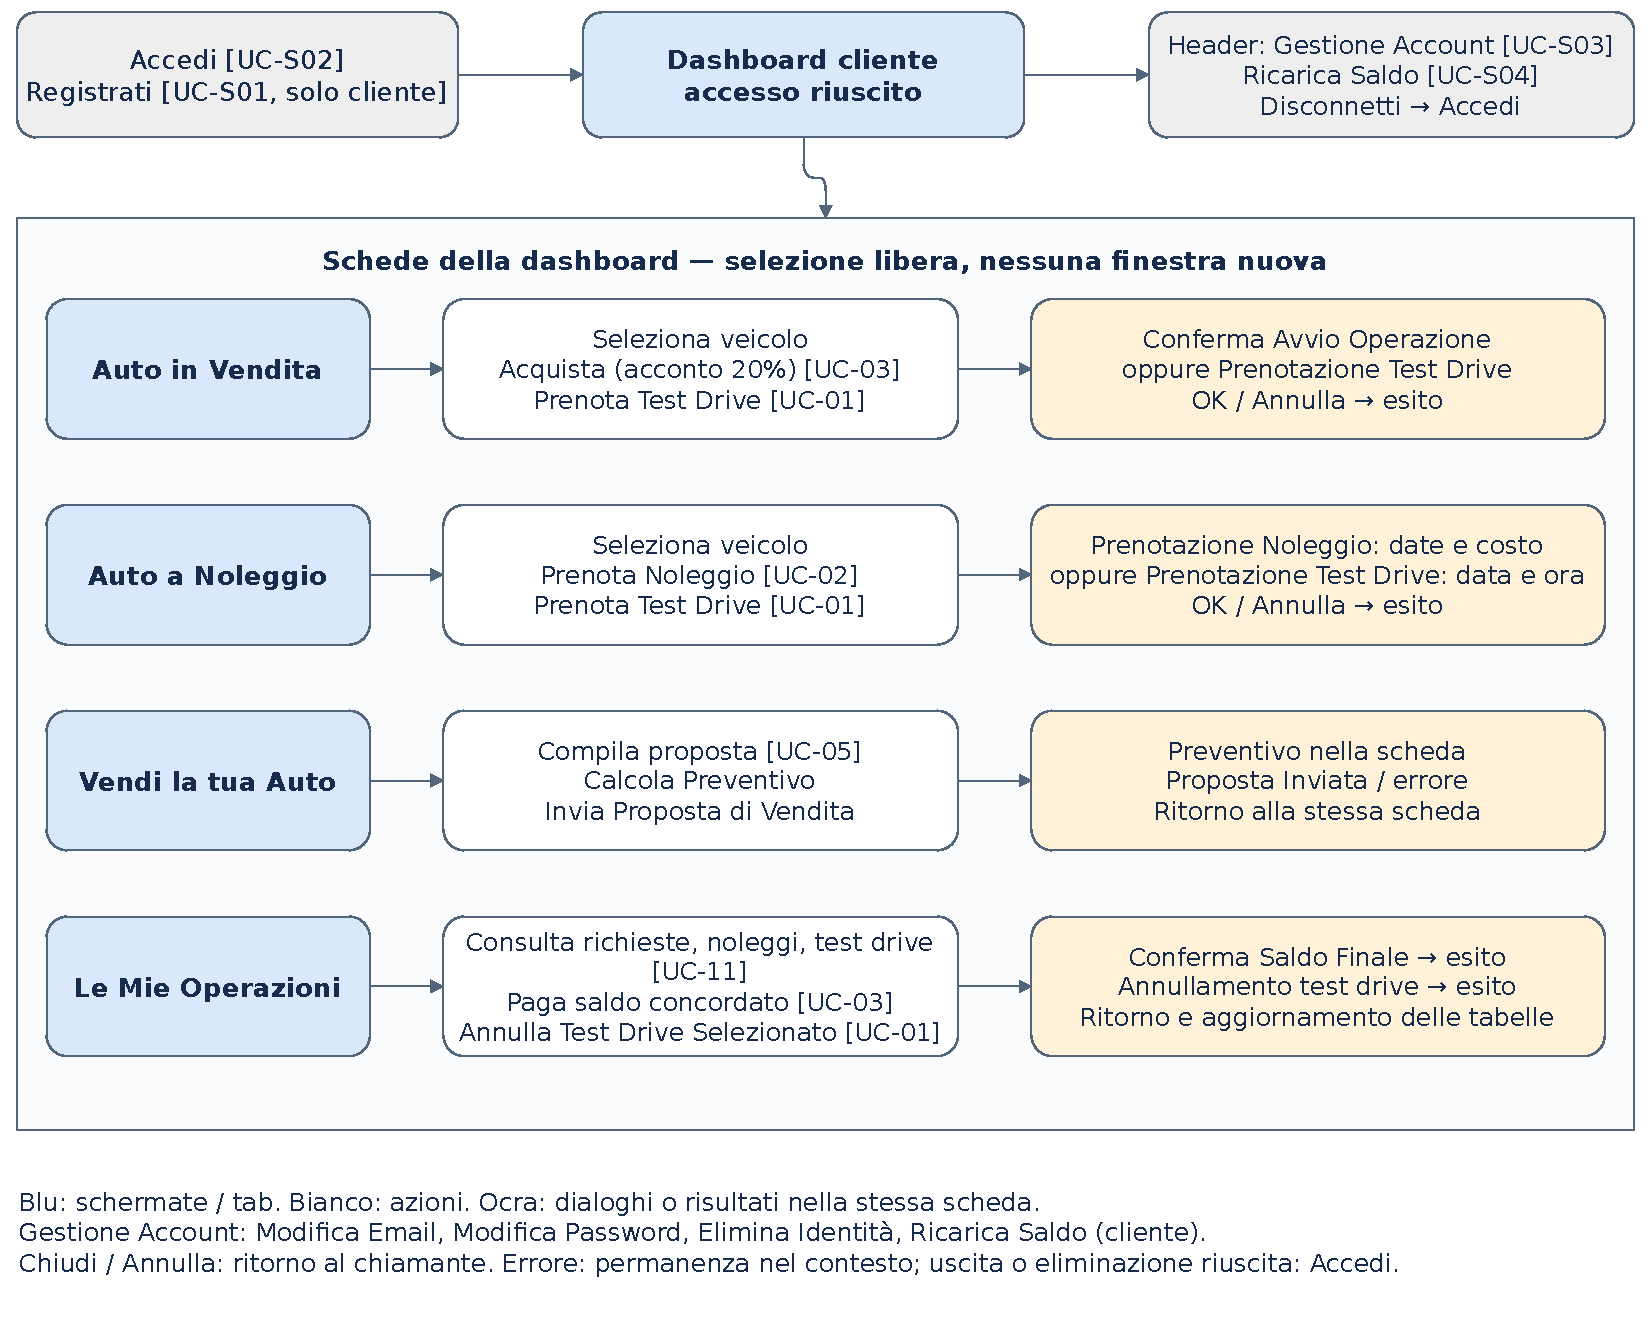
\includegraphics[width=\linewidth,height=.7\textheight,keepaspectratio]{diagrammi/navigazione-cliente.drawio.pdf}
\caption{Navigazione cliente: quattro tab; dialoghi di prenotazione, acconto e saldo; proposta nella scheda; gestione identit\`a e conto. Riscontri visivi nelle figure~\ref{fig:ui-cliente-catalogo}--\ref{fig:ui-identita}.}\label{fig:nav-cliente}
\end{figure}
\clearpage
\begin{figure}[!htbp]\centering
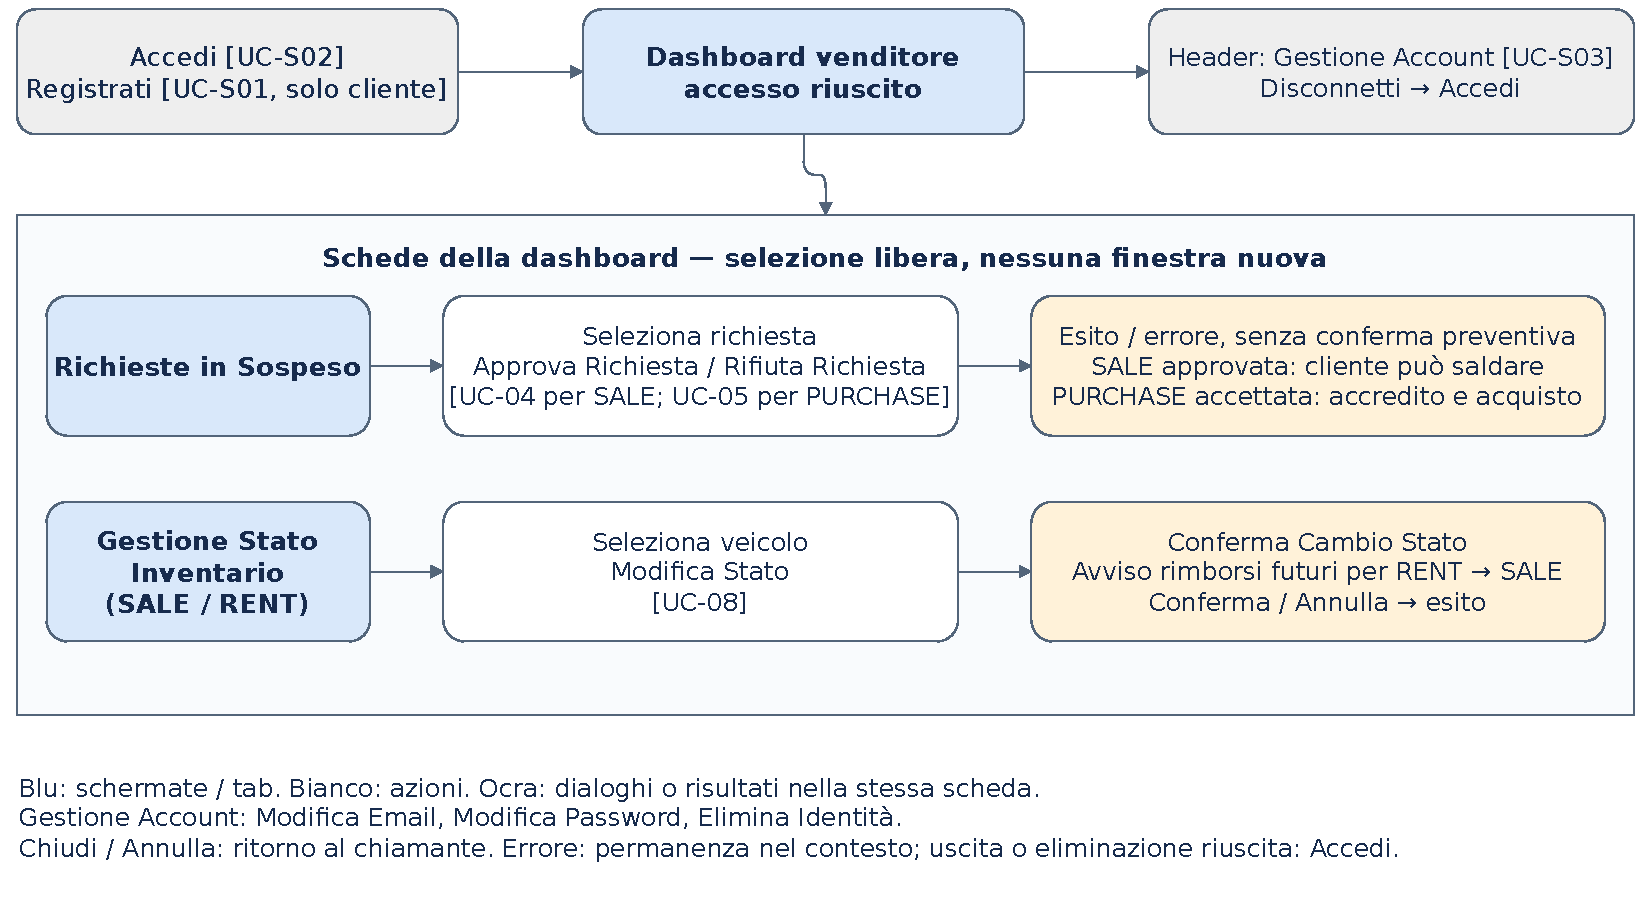
\includegraphics[width=\linewidth,height=.72\textheight,keepaspectratio]{diagrammi/navigazione-venditore.drawio.pdf}
\caption{Navigazione venditore: richieste ed inventario, corrispondenti alle figure~\ref{fig:ui-venditore-richieste} e~\ref{fig:ui-venditore-inventario}. L'approvazione non apre una conferma preventiva; il cambio destinazione s\`i.}\label{fig:nav-venditore}
\end{figure}
Le azioni \emph{Approva Richiesta} e \emph{Rifiuta Richiesta} hanno esiti diversi
secondo il tipo della riga. Una richiesta di vendita al cliente approvata
rimanda il completamento al cliente; l'accettazione di una cessione effettua
subito accredito e acquisto. Il cambio destinazione mostra un avviso dei
noleggi futuri, ma il servizio ne rilegge lo stato prima del commit.
\clearpage
\begin{figure}[!htbp]\centering
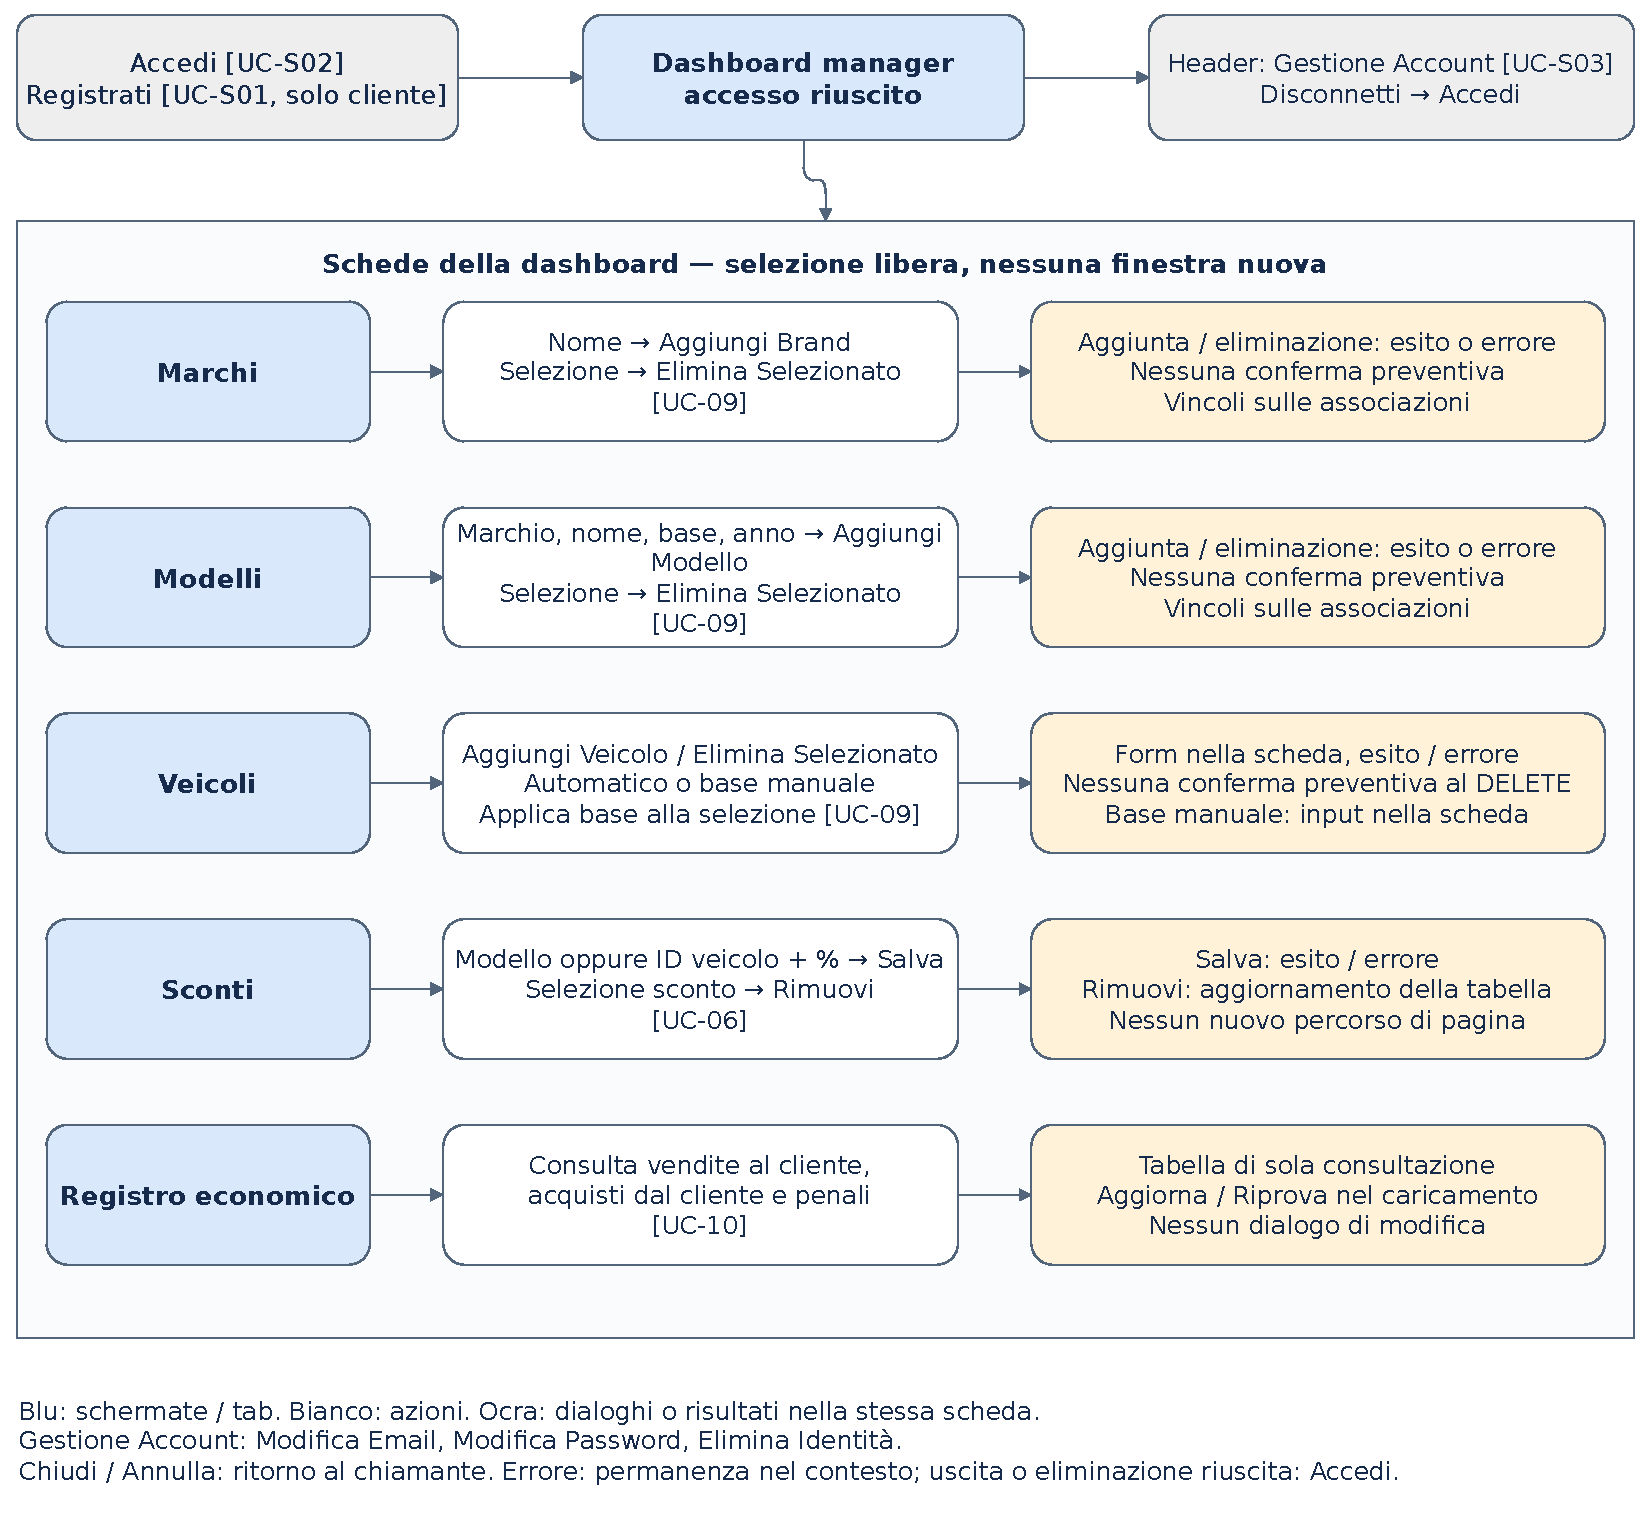
\includegraphics[width=\linewidth,height=.76\textheight,keepaspectratio]{diagrammi/navigazione-manager.drawio.pdf}
\caption{Navigazione manager: cinque tab e form nella stessa vista, corrispondenti alle figure~\ref{fig:ui-manager-marchi}--\ref{fig:ui-manager-registro}. Il registro \`e di sola consultazione.}\label{fig:nav-manager}
\end{figure}
Le rimozioni di catalogo e sconti sono azioni dirette; la vista non aggiunge
una conferma preventiva. Durante le letture asincrone di cataloghi, inventario,
sconti e registro i dati sono disabilitati; in caso di errore compare
\emph{Riprova}. Questo comportamento non va esteso alle letture sincrone
di richieste e operazioni personali. Le nuove tavole sono conservate con
sorgenti \code{.drawio} ed esportazioni PDF in \code{docs/relazione/diagrammi}.
\clearpage

\endgroup

\begingroup
\emergencystretch=6em
\def\UrlBreaks{\do\a\do\b\do\c\do\d\do\e\do\f\do\g\do\h\do\i\do\j\do\k\do\l\do\m\do\n\do\o\do\p\do\q\do\r\do\s\do\t\do\u\do\v\do\w\do\x\do\y\do\z\do\A\do\B\do\C\do\D\do\E\do\F\do\G\do\H\do\I\do\J\do\K\do\L\do\M\do\N\do\O\do\P\do\Q\do\R\do\S\do\T\do\U\do\V\do\W\do\X\do\Y\do\Z}
\section{Package Diagram}\label{sec:package}
L'organizzazione corrente comprende undici package con tipi di produzione.
La figura~\ref{fig:pkg} distingue la composizione dell'applicazione dai suoi
collaboratori: le frecce indicano chi dipende da chi nel codice, non il verso
di restituzione dei dati. I package intermedi \code{domain} e
\code{presentation} non contengono tipi propri e non richiedono viste vuote.

\code{App} avvia JavaFX e collega utente, servizi e callback alle viste;
\code{AppContext} costruisce i DAO PostgreSQL, il gestore delle connessioni,
l'hasher, il publisher con il suo observer e i servizi. Questa composizione
manuale concentra le scelte concrete senza un container. Il contesto riceve
un \code{DatabaseManager}, ma sceglie internamente le implementazioni:
non rende quindi sostituibile ogni dipendenza dal solo costruttore.

\subsection*{Il dominio non dipende dagli altri livelli}
I servizi coordinano i casi d'uso delle sezioni precedenti. Dipendono dai
contratti DAO e dal dominio; i servizi transazionali conoscono anche
\code{DatabaseManager} e JDBC. I DAO definiscono letture, scritture e lock
per risorsa; \code{dao.postgres} ne realizza mapping e SQL. Il dominio
non richiama i DAO e i suoi quattro package non importano gli altri
package applicativi. Ciò non equivale a un isolamento completo dalle
esigenze dell'interfaccia: \code{domain.user} contiene il contratto di
navigazione per ruolo.

\tavolaautori{package-autori}{Package correnti: struttura degli autori e dipendenze attuali}{fig:pkg}
\clearpage

Le dipendenze trasversali limitano una lettura rigidamente a strati.
Le viste usano servizi concreti e tipi del dominio; gli overload di comodo
richiamano il contesto globale, mentre \code{App} passa esplicitamente i
servizi. \code{service} dipende da \code{event}, anche attraverso la
realizzazione dell'observer, ma \code{event} non dipende da \code{service}:
conosce solo il contratto degli osservatori. La connessione JDBC attraversa
questa notifica. \code{security} offre hash e verifica delle password a
\code{AuthService}; non concentra l'autorizzazione di tutte le operazioni.
Le note della tavola completano gli archi selezionati e rendono visibile
anche la dipendenza reciproca tra package di avvio e presentazione.

La separazione evita SQL nelle viste e concentra le formule nel calcolatore,
ma lascia responsabilità ampie nelle dashboard e in \code{AuthService},
che tratta accesso, identità e conto dimostrativo. I contratti che espongono
\code{Connection} facilitano la condivisione della transazione, al prezzo
di legare anche i servizi a JDBC. Non si attribuisce al sistema
un'architettura esagonale o una separazione ideale assente dai sorgenti.

\section{Class Diagram}\label{sec:classi}
Le viste selezionano responsabilità, invarianti e collaborazioni: non sono
cataloghi di tutti i membri. L'appendice~\ref{app:classi} raccoglie le tavole
CL-01--CL-11, con due tavole CL-08a e CL-08b per il package DAO.
Gli identificativi rimangono gli stessi nei rimandi e nei sorgenti draw.io.

La legenda distingue generalizzazione (linea continua e triangolo vuoto),
realizzazione (tratteggio e triangolo), dipendenza (tratteggio e freccia
aperta) e associazione navigabile (linea continua e freccia aperta).
Le molteplicità annotate si riferiscono al solo estremo bersaglio;
l'altro estremo non impone un vincolo numerico. Non sono impiegati rombi
di aggregazione o composizione: un campo o l'iniezione di un collaboratore
non ne dimostrano il ciclo di vita. Gli attributi marcati \code{ID} o
\code{chiave} restano riferimenti scalari, non associazioni a oggetti.

\subsection{Domain Model}
Il dominio separa identità, catalogo, sconti e operazioni. Nella gerarchia
degli utenti, \code{AbstractUser} realizza \code{User}; \code{Client},
\code{Salesman} e \code{Manager} specializzano la parte comune.
\code{Client} può conservare un \code{BankAccount} oppure non averlo ancora
caricato: CL-02 mostra quindi una navigazione verso zero o un conto.
Il conto conserva a sua volta soltanto \code{clientId}; non si disegna
un collegamento inverso a \code{Client}. Il suo comportamento controlla
importi e disponibilità nel modello dimostrativo, non integra una banca.

La figura~\ref{fig:catalogo-corpo} mostra una distinzione utile anche per
UC-03 e UC-09: un veicolo conserva \code{modelId}, mentre riceve un oggetto
\code{Model} quando deve scegliere la base del prezzo. Il primo è un
riferimento per ID; il secondo giustifica una dipendenza di metodo.
Analogamente \code{Model.brand} è una stringa, non un oggetto \code{Brand}.
Stato e modalità del prezzo sono invece attributi tipizzati dagli enum.
La base manuale entra nella stessa formula della base modello, come
stabilito dall'ADR~0001; il totale concordato è un concetto distinto.

\tavolaautori{classi-dominio-insieme}{Domain Model d'insieme: utenti, catalogo, sconti e operazioni}{fig:catalogo-corpo}
\clearpage

CL-04 rende esplicita la sola generalizzazione degli sconti: il limite
intero 0--50 appartiene alla base astratta, mentre le specializzazioni
conservano l'ID del modello o del veicolo. La scelta dello sconto massimo
è responsabilità del servizio di calcolo, non di una relazione tra entità.
CL-05 distingue \code{Request} dal registro \code{Sale} e dalle prenotazioni
\code{Rent}/\code{TestDrive}. Nessuna di queste classi contiene oggetti
cliente o veicolo. Le richieste \code{SALE} conservano totale e acconto
dell'accordo di UC-03; nelle \code{PURCHASE}, relative a UC-05, il campo
\code{deposit} contiene la stima e il totale concordato è assente.
Il tipo del registro distingue vendita al cliente, acquisto dal cliente e penale con importi
non negativi, senza dedurre il significato dal segno.

\subsection{Business Layer}
CL-01 e CL-06 separano composizione e coordinamento. Il contesto conserva
i collaboratori e li passa ai costruttori. I tre servizi dei flussi
economici coordinano i DAO, mentre il calcolatore concentra le formule.
\code{CatalogService} prepara anche righe con nomi e prezzi per le tabelle;
il servizio di interrogazione espone le letture delle operazioni.
I record annidati del catalogo sono dati di lettura, non nuove entità persistenti.

L'observer di cancellazione appartiene a \code{service}, perché applica
la priorità della vendita al cliente e del noleggio sui test drive di UC-01.
Il contratto, il publisher e l'evento risiedono invece in \code{event}.
La figura~\ref{fig:eventi-corpo} comprende la collaborazione di notifica sincrona sulla connessione
del servizio prima del commit: un errore dell'observer deve impedirlo.
La separazione consente altri osservatori, ma non offre consegna asincrona,
persistenza degli eventi o recupero tramite outbox.

\tavolaautori{classi-business-insieme}{Business Layer d'insieme: servizi, calcolo, transazioni, sicurezza ed eventi}{fig:eventi-corpo}
\clearpage

\subsection{DAO}
CL-08a raccoglie dieci contratti distinti per risorsa, senza un gestore
comune da cui ereditare. La classe \code{DatabaseManager} apre connessioni ed esegue il corpo
di una transazione mediante le due callback annidate di CL-08b, tentando
commit oppure rollback in caso di eccezione. Non è un DAO base né un ORM.
Le firme con \code{Connection} rendono visibile la partecipazione di più
scritture alla stessa transazione. Alcuni overload di lettura dei contratti
forniscono però un default che delega alla lettura senza connessione:
la sola firma non basta a garantirne il riuso. I DAO PostgreSQL pertinenti
ridefiniscono tali percorsi.

CL-09 rende riconoscibile ciascuna realizzazione del relativo contratto.
Ogni DAO PostgreSQL conserva il gestore ricevuto dal costruttore: non si
deduce una composizione UML da questo riferimento condiviso. Le letture
autonome gestiscono la propria connessione; quelle transazionali e le
scritture protette usano quella passata dal servizio. Il mapping ricostruisce
le entità e converte i domini enumerati in accordo con l'ADR~0002.
Gli ID che legano i record persistenti non diventano per questo riferimenti
a oggetti nel dominio. I dettagli SQL e i protocolli dei singoli flussi
sono rinviati al capitolo~\ref{ch:implementazione}.


\tavolaautori{classi-dao-insieme}{DAO d'insieme: contratti, realizzazioni PostgreSQL e gestore JDBC}{fig:dao-insieme}
\clearpage

\subsection{Presentation Layer}
CL-10 mostra le viste effettive: accesso e tre dashboard estendono
\code{BorderPane}; il dialogo di gestione dell'identità è una classe di
utilità con metodi statici, non un sottotipo di \code{Dialog}. Le viste
costruiscono controlli JavaFX direttamente, senza controller FXML.
\code{AsyncLoad}, interno al package, usa \code{Task} e worker virtuali
per le letture delle tabelle; pubblica solo il caricamento corrente sul
thread grafico. Ciò non rende asincrone tutte le azioni economiche né
interrompe immediatamente JDBC quando un caricamento è scartato.

La navigazione delle sezioni 2.3--2.4 parte da \code{User}: il suo metodo
\code{openDashboard} viene specializzato nei tre ruoli. Il sottotipo invoca
il metodo specifico del contratto \code{UserDashboardNavigator}.
\code{App} crea un'implementazione anonima
che costruisce la dashboard appropriata. È un double dispatch nello
stile Visitor: aggiungere un ruolo richiede di aggiornare anche il
contratto e il collegamento delle viste. \code{App} non realizza direttamente
quell'interfaccia. Il dominio resta privo di import JavaFX, ma conosce
questa esigenza di navigazione.

CL-11 mostra il confine delle credenziali. Il contratto
\code{PasswordHasher} è ricevuto da \code{AuthService}; la realizzazione
PBKDF2 viene scelta nel contesto.
Questo confine riguarda hash e verifica della password. La scelta della
dashboard per ruolo non equivale a un controllo autonomo dei permessi
in ogni metodo dei servizi, che non ricevono tutti un'identità autenticata.
Non viene quindi attribuita al solo package \code{security} una garanzia
generale di autorizzazione.
\clearpage

\tavolaautori{classi-presentazione-insieme}{Presentazione d'insieme: viste, dialogo comune e navigazione}{fig:presentazione-insieme}
\clearpage

\endgroup

\section{Sequence Diagram}
\subsection{Acquisto di un veicolo}
\provvisorio{Descrivere la vendita al cliente: acconto, esito della richiesta e saldo.}
\subsection{Prenotazione di un noleggio}
\provvisorio{Descrivere prenotazione, conflitti e cancellazioni collegate dei test drive.}
\subsection{Acquisizione di un veicolo del Customer}
\provvisorio{Descrivere l'acquisto dal cliente: proposta, esito e registrazione economica.}

\section{Database}
\subsection{Schema ER}
\provvisorio{Inserire il modello ER dello schema PostgreSQL corrente.}
\subsection{Modello relazionale}
\provvisorio{Documentare relazioni, cardinalità, chiavi e domini enumerati.}
\subsection{Utenti, vincoli e semplificazioni}
\provvisorio{Spiegare vincoli effettivi e limiti del modello dei dati.}
